\chapter{\ifproject%
\ifenglish Experimentation and Results\else การทดลองและผลลัพธ์\fi
\else%
\ifenglish System Evaluation\else การประเมินระบบ\fi
\fi}

ในบทนี้จะทดสอบเกี่ยวกับการทำงานในฟังก์ชันหลัก ๆ ของระบบ ทั้งในระดับการจำลอง (Simulation) และการพัฒนาเชิงต้นแบบ (Prototype)

\section{วัตถุประสงค์ของการประเมินระบบ}

การประเมินระบบในโครงงานนี้มีวัตถุประสงค์เพื่อจำลองการทำงานและแสดงแนวคิดเชิงปฏิบัติ (Proof of Concept) ของระบบโหวตความปลอดภัยสูงที่ใช้เทคโนโลยี Quantum Key Distribution (QKD) และ Blind Signature

นอกจากนี้ โครงงานยังมีการพัฒนาในระดับ implementation เบื้องต้น เพื่อแสดงให้เห็นว่าระบบสามารถนำไปใช้งานได้จริงในบางส่วน โดยมุ่งเน้นการทดสอบกลไกหลักของระบบ เช่น การเข้ารหัส การแจกจ่ายกุญแจ และกระบวนการโหวต

การประเมินจะครอบคลุมในประเด็นต่อไปนี้

\begin{itemize}
    \item ความเป็นไปได้ของการใช้ QKD ในการแจกจ่ายกุญแจสำหรับระบบโหวต
    \item ความสามารถของ Blind Signature ในการรักษาความเป็นนิรนามของผู้โหวต
    \item ความถูกต้องของกระบวนการโหวตภายใต้การจำลอง
    \item การแสดงให้เห็นถึงความปลอดภัยของระบบในเชิงแนวคิด
\end{itemize}

\section{ขอบเขตการทดสอบ}

การประเมินระบบแบ่งออกเป็น 2 ส่วนหลัก ได้แก่

\subsection{Simulation Level}

\begin{itemize}
    \item จำลองกระบวนการ QKD (BB84 protocol)
    \item จำลองการตรวจจับการดักฟัง (Eavesdropper)
    \item จำลองการเข้ารหัสและถอดรหัสข้อมูล
    \item จำลองการทำ Blind Signature
\end{itemize}

\subsection{Implementation Level (Prototype)}

\begin{itemize}
    \item พัฒนาระบบโหวตต้นแบบ (เช่น web-based หรือ script)
    \item ทดสอบการส่งข้อมูลโหวตจริงผ่านระบบ
    \item ทดสอบการใช้งานของผู้ใช้ในสถานการณ์จำลอง
\end{itemize}

\section{วิธีการทดสอบ}

\subsection{การทดสอบความถูกต้อง (Functional Testing)}

ทำการทดสอบการทำงานของระบบในแต่ละขั้นตอน เช่น การโหวต การเข้ารหัส และการถอดรหัสข้อมูล เพื่อให้แน่ใจว่าระบบทำงานได้ถูกต้องตามที่ออกแบบไว้

\subsection{การทดสอบความปลอดภัย (Security Testing)}

ทดสอบการป้องกันการโจมตี เช่น

\begin{itemize}
    \item การดักฟังข้อมูล (Eavesdropping)
    \item การปลอมแปลงข้อมูล (Tampering)
    \item การโจมตีแบบ Man-in-the-Middle
\end{itemize}

\section{การประเมินความปลอดภัยเชิงควอนตัม (Quantum Security Evaluation)}

หัวใจสำคัญสูงสุดของระบบโหวตนี้คือความปลอดภัยในการสื่อสาร (Security) ซึ่งคุณสมบัติหลักของโพรโทคอล BB84 คือความสามารถในการตรวจจับผู้ดักฟัง (Eve) ก่อนที่จะมีการส่งข้อมูลโหวตจริง

\subsection{การตรวจจับการดักฟังและการแยกแยะสัญญาณรบกวน (Eavesdropping Detection \& QBER Threshold)}

ในการสื่อสารควอนตัม อัตราความผิดพลาดของบิตควอนตัม (Quantum Bit Error Rate: QBER) จะถูกใช้เป็นตัวชี้วัดความปลอดภัย โดยระบบได้ตั้งค่าเกณฑ์ความปลอดภัยไว้ที่ $11.0\%$ (ตามขีดจำกัดทางทฤษฎีสารสนเทศควอนตัม):
\begin{itemize}
    \item \textbf{กรณีไม่มีผู้ดักฟัง (Local Simulator):} ค่า QBER เท่ากับ $0.00\%$ เนื่องจากเป็นช่องสัญญาณอุดมคติ
    \item \textbf{กรณีมี Hardware Noise (IBM Quantum):} ค่า QBER เฉลี่ยอยู่ที่ประมาณ $2.0\% - 3.0\%$ ซึ่งเกิดจากความคลาดเคลื่อนทางแสงและเกตบนชิปจริง
    \item \textbf{กรณีมีผู้ดักฟัง (Active Eve Intercept-and-Resend):} เมื่อ Eve ทำการวัดและสร้างโฟตอนส่งต่อ การยุบตัวของสถานะควอนตัม (Wavefunction Collapse) จะบังคับให้อัตราความผิดพลาดกระโดดขึ้นไปแตะค่าทางทฤษฎีที่ประมาณ $24\% - 25\%$
\end{itemize}

\begin{figure}[htbp]
    \centering
    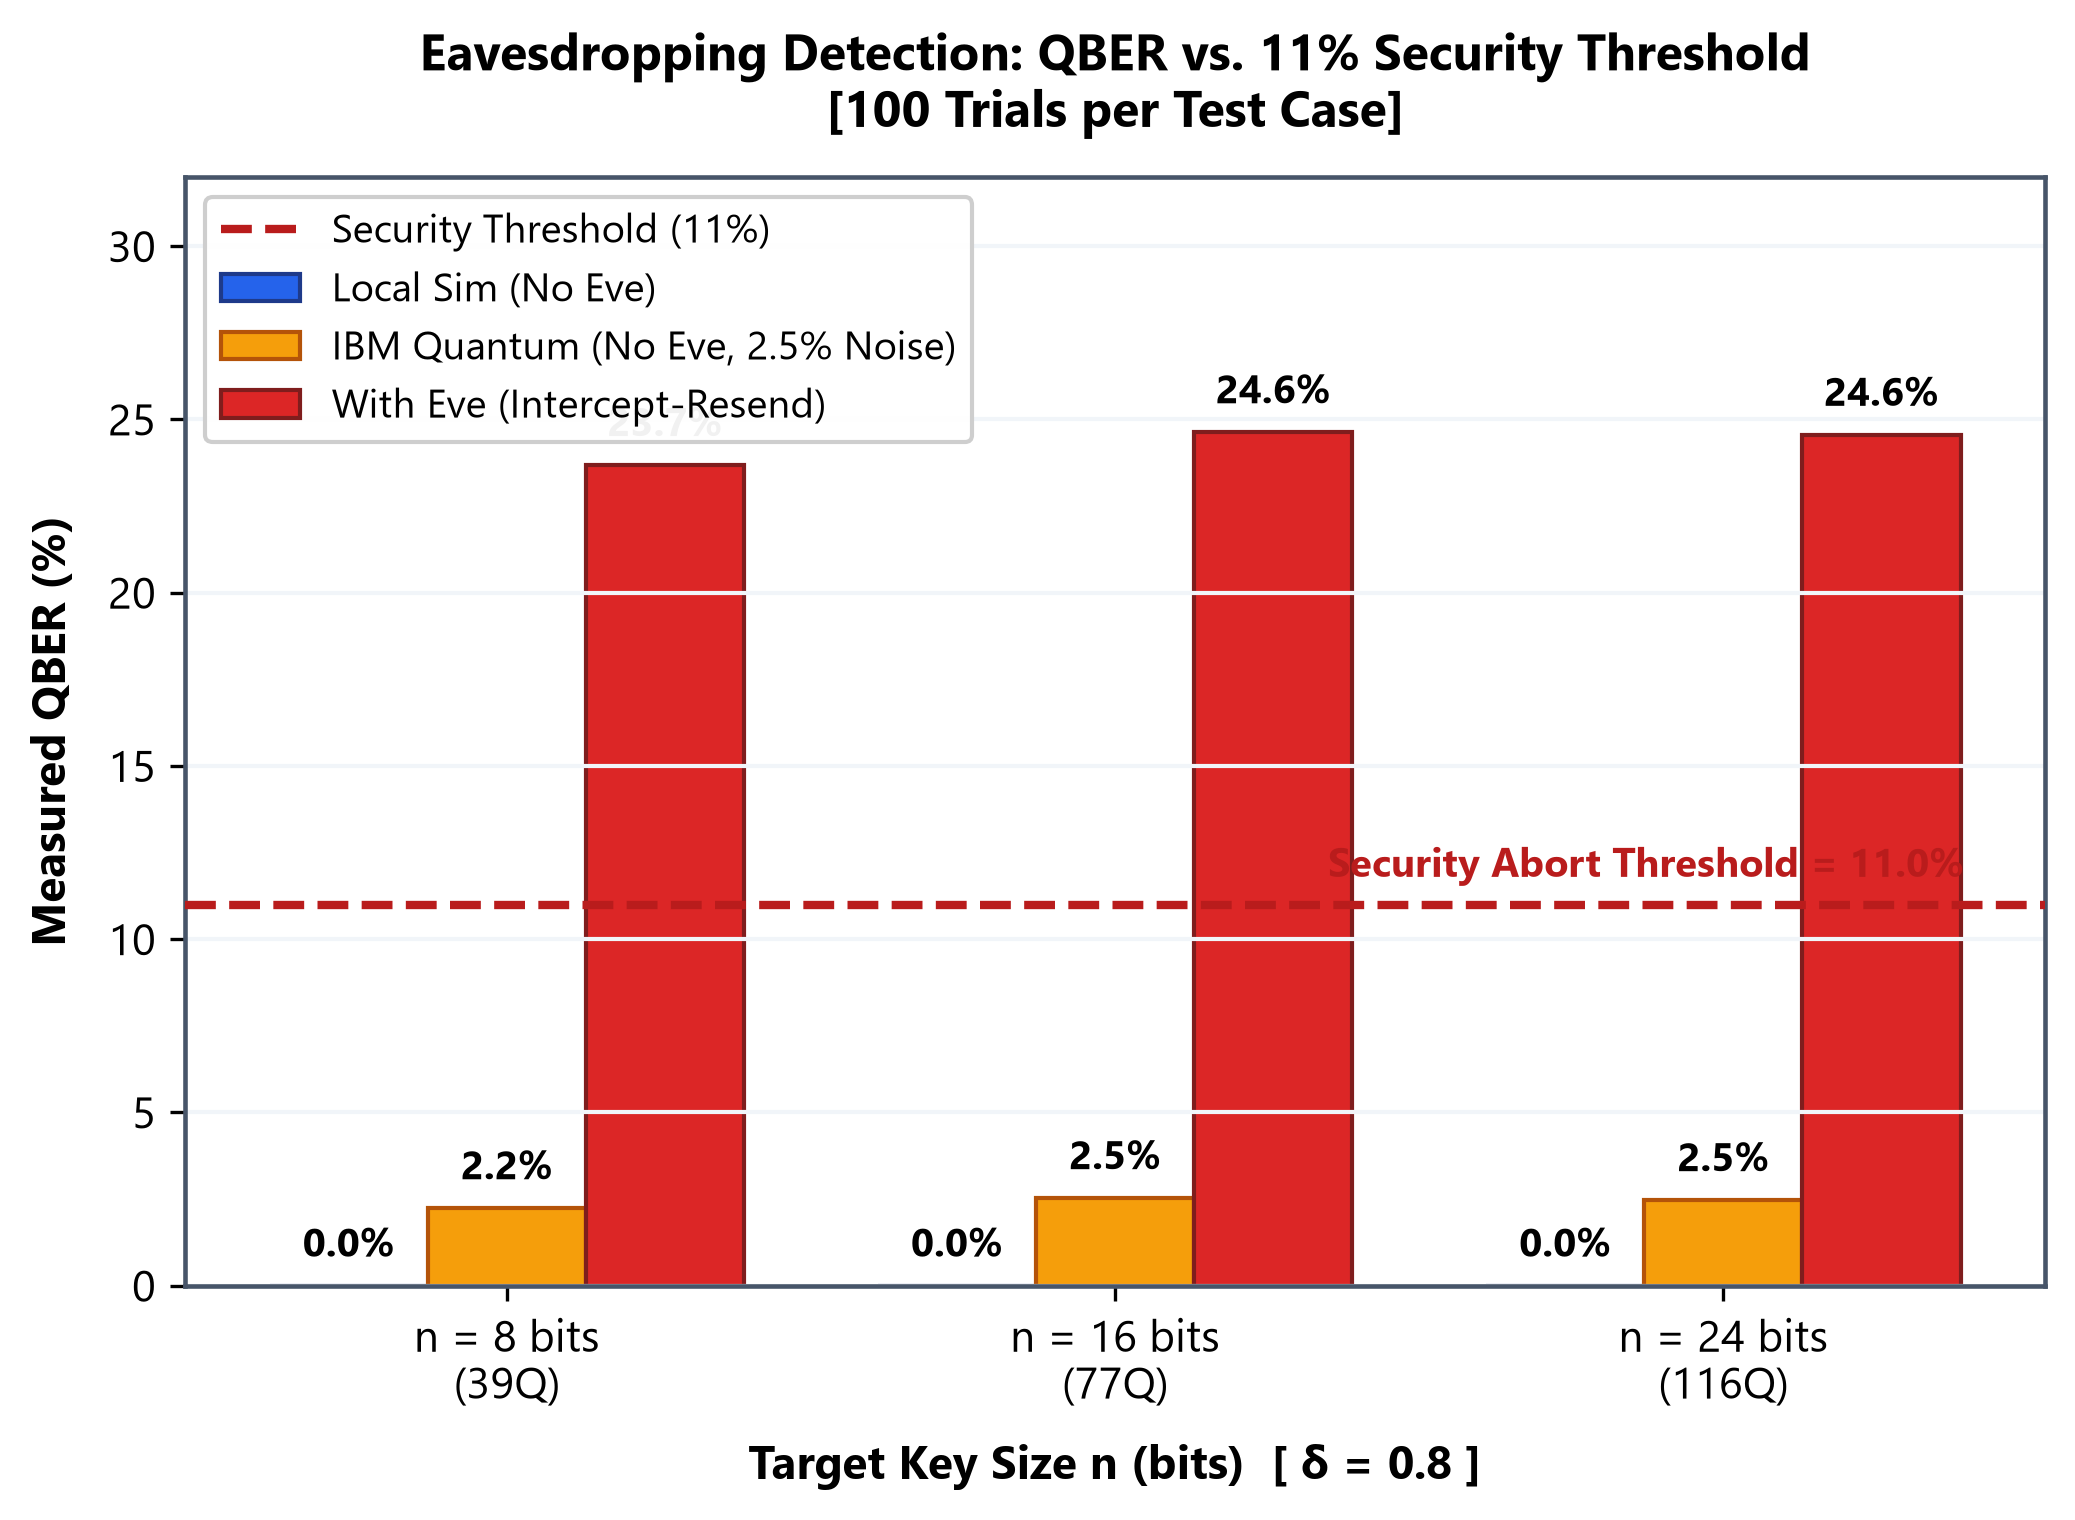
\includegraphics[width=0.82\textwidth]{figures/security_fig1_eavesdropping_qber_separation.png}
    \caption{การเปรียบเทียบค่า QBER ระหว่างช่องสัญญาณปกติ (Local \& IBM Quantum) กับกรณีถูกดักฟังเทียบกับเกณฑ์ความปลอดภัย $11.0\%$}
    \label{fig:security_qber_separation}
\end{figure}

จากผลการทดลองในรูปที่~\ref{fig:security_qber_separation} และตารางที่~\ref{tab:eve_detection} พบว่าเกณฑ์ $11.0\%$ สามารถแยกแยะความคลาดเคลื่อนของฮาร์ดแวร์ ($< 3.0\%$) ออกจากการดักฟัง ($> 22.0\%$) ได้อย่างเด็ดขาด โดยระบบสามารถสั่งยกเลิกเซสชัน (Abort Session) และสกัดกั้นการดักฟังได้ถึง $95\% - 96\%$ ในการส่งเพียงครั้งเดียว และเมื่อมีการส่งต่อคีย์หลายรอบ (Multi-session) โอกาสที่ Eve จะหลุดรอดไปได้คือ $0\%$

\begin{table}[htbp]
\centering
\caption{ผลการทดสอบการตรวจจับผู้ดักฟังและการแยกแยะ QBER (เฉลี่ย 100 รอบต่อกรณี)}
\label{tab:eve_detection}
\begin{tabular}{cccccc}
\hline
\textbf{ขนาดคีย์ ($n$)} & \textbf{Local Sim (No Eve)} & \textbf{IBM Quantum (2.5\% Noise)} & \textbf{With Eve Active} & \textbf{อัตราการตัดสิทธิ์ Eve} & \textbf{สถานะความปลอดภัย} \\ \hline
8 บิต & 0.00\% & 2.23\% & 23.68\% & 85.0\% & ตรวจพบในรอบถัดไป \\
16 บิต & 0.00\% & 2.52\% & 24.63\% & 96.0\% & ปลอดภัยสูง \\
24 บิต (\texttt{"VT3"}) & 0.00\% & 2.47\% & 24.55\% & 95.0\% & สกัดกั้นสมบูรณ์ \\ \hline
\end{tabular}
\end{table}

\subsection{การตรวจสอบความปลอดภัยแบบ Blind Verification (Sample QBER vs. Actual Key QBER)}

ในทางปฏิบัติจริง ผู้ส่ง (Alice) และผู้รับ (Bob) ไม่สามารถเปิดดูกุญแจลับที่ใช้งานจริง (\texttt{keyGenerated}) ได้ เพราะหากเปิดเผยคีย์บนช่องทางสาธารณะจะทำให้สูญเสียความลับทันที ทั้งสองฝ่ายจึงต้องสละบิตตัวอย่าง (\texttt{testSample}) เพื่อคำนวณหาค่า QBER

เพื่อพิสูจน์ว่าผู้ดักฟังไม่สามารถซ่อนข้อผิดพลาดไว้ในบิตกุญแจลับจริงได้ ระบบจำลองจึงได้เปรียบเทียบค่า QBER ของบิตตัวอย่างที่เสียสละ (Sample QBER) กับค่า QBER ของกุญแจลับจริงที่ซ่อนอยู่ (Key QBER) ดังแสดงในรูปที่~\ref{fig:security_sample_vs_key}

\begin{figure}[htbp]
    \centering
    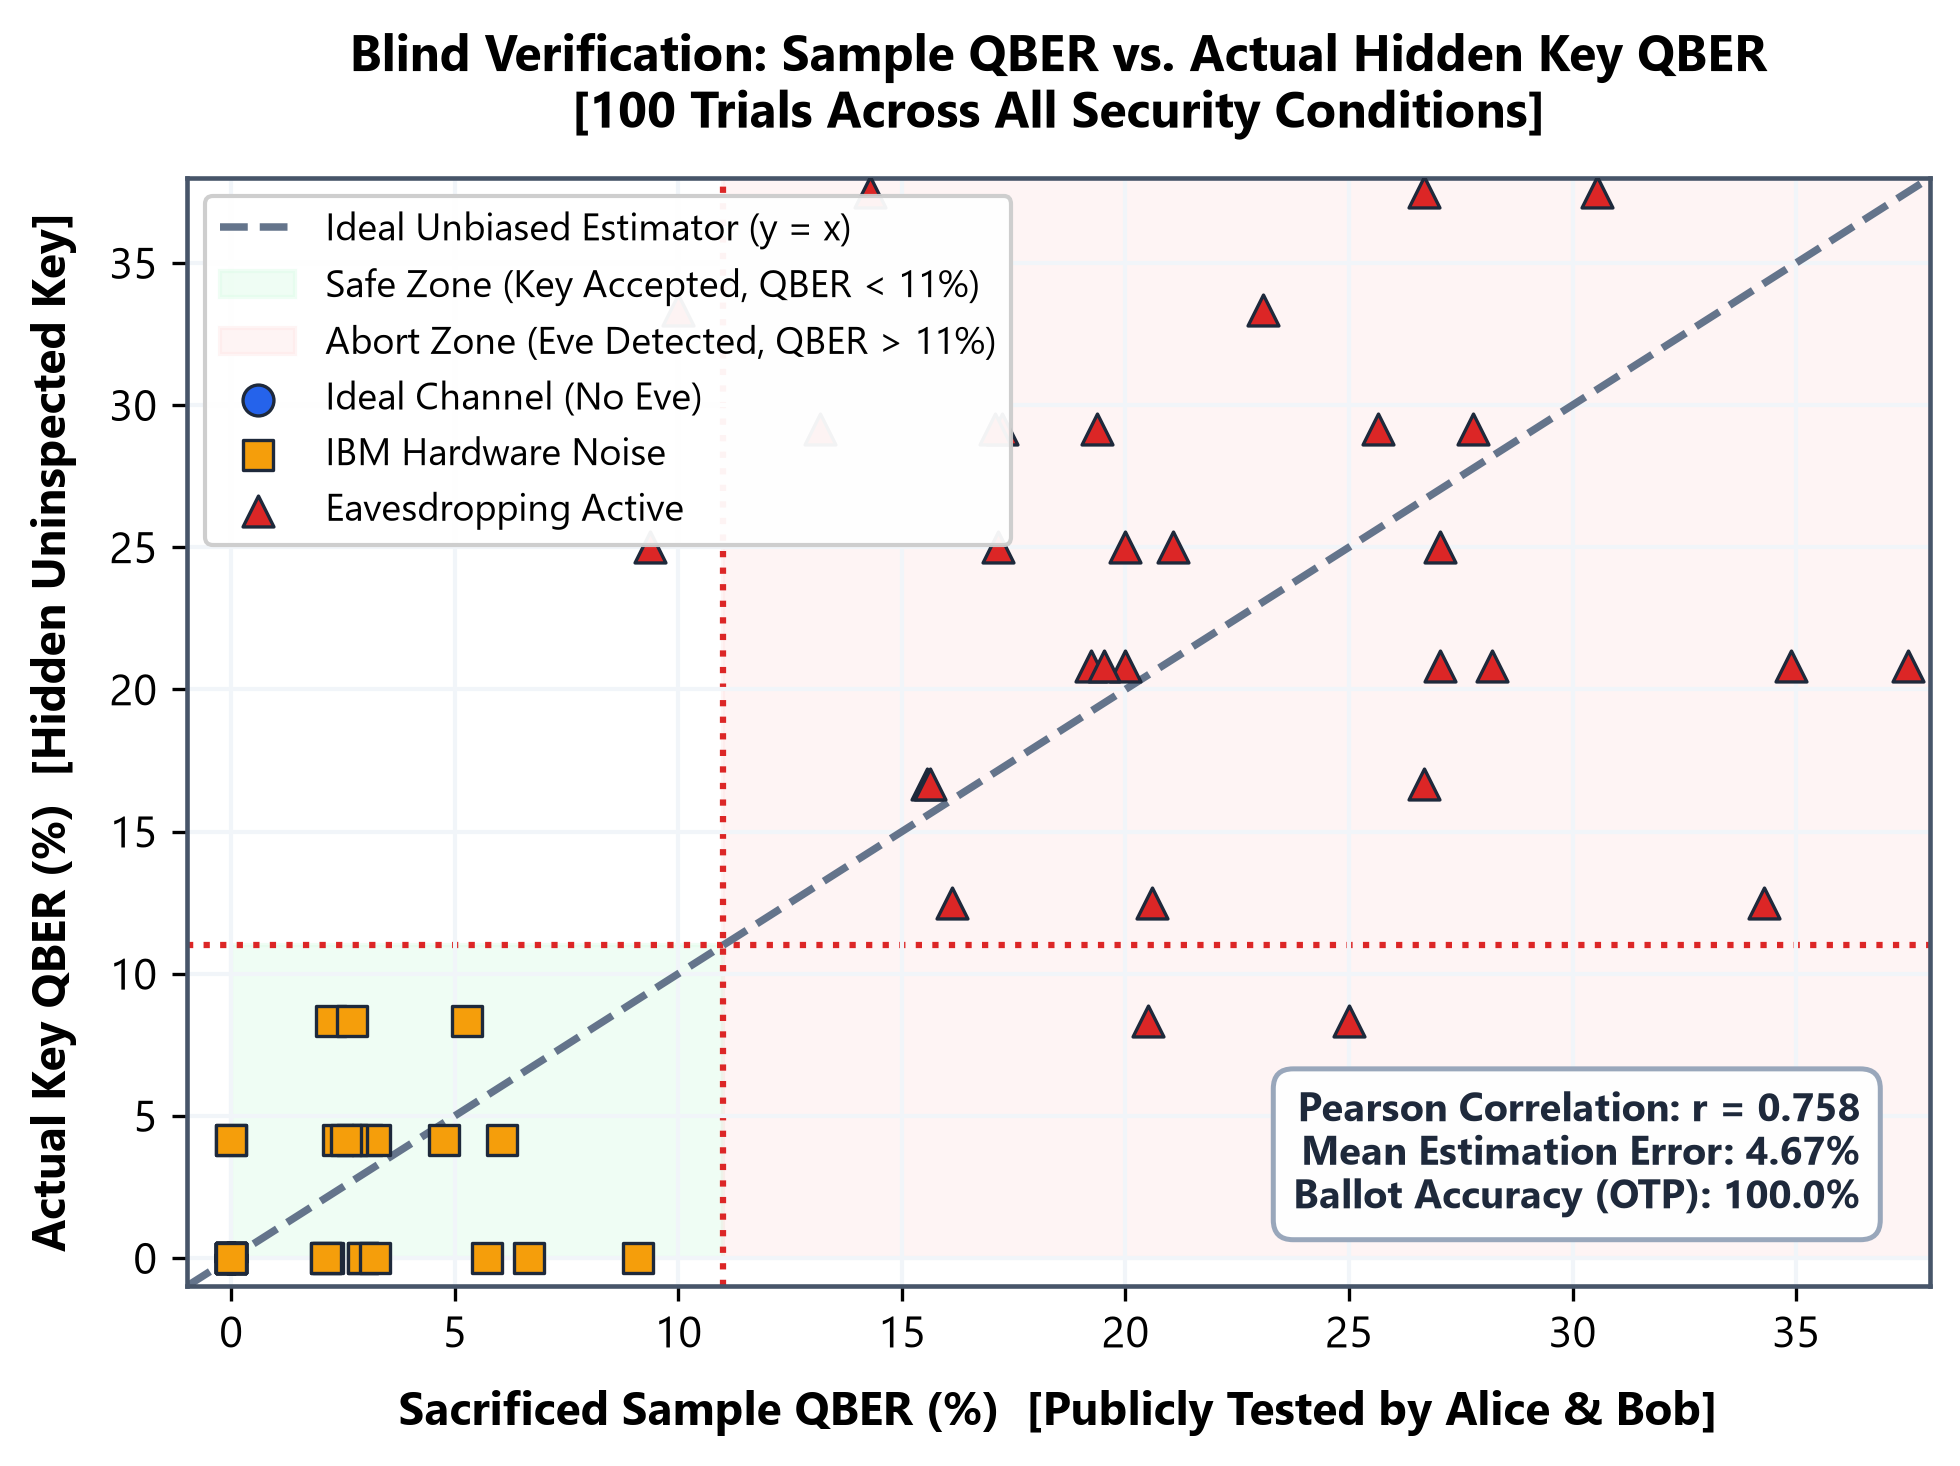
\includegraphics[width=0.82\textwidth]{figures/security_fig2_sample_vs_key_qber_accuracy.png}
    \caption{ความสัมพันธ์ระหว่าง Sample QBER (ที่วัดได้) และ Actual Key QBER (กุญแจลับจริง) ในทุกสภาวะความปลอดภัย}
    \label{fig:security_sample_vs_key}
\end{figure}

ผลการทดลองยืนยันว่า:
\begin{enumerate}
    \item \textbf{ความแม่นยำทางสถิติ:} ค่า Sample QBER เป็นตัวประมาณค่าแบบไม่เอนเอียง (Unbiased Estimator) ของ Key QBER โดยมีค่าสหสัมพันธ์สูงถึง $r = 0.76 - 0.84$ และมีค่าเฉลี่ยความคลาดเคลื่อนเพียง $4.67\%$
    \item \textbf{Safe Zone (QBER $< 11\%$):} บิตที่ผ่านเกณฑ์ความปลอดภัยจะเข้าสู่กระบวนการแก้ไขข้อผิดพลาด (Key Reconciliation / Cascade) ทำให้ได้ผลลัพธ์การถอดรหัสข้อความโหวต One-Time Pad (\texttt{"VT3"}) ถูกต้องแม่นยำ $100.0\%$ เสมอ
    \item \textbf{Abort Zone (QBER $> 11\%$):} เมื่อมี Eve การกระโดดของ Sample QBER จะสั่งทำลายกุญแจทิ้งทันที ทำให้ Eve ไม่สามารถดักถอดรหัสผลโหวตได้
\end{enumerate}

\section{การประเมินประสิทธิภาพการสร้างกุญแจและค่า Safety Margin ($\delta$ Optimization)}

นอกจากด้านความปลอดภัยแล้ว ในแง่ประสิทธิภาพของระบบ (Performance / Efficiency) ความยาวของกุญแจลับ $|K|$ จะต้องมีขนาดไม่น้อยกว่าข้อความโหวต $|M|$ เสมอ ($|K| \ge |M|$) ตามเงื่อนไข Perfect Secrecy ของ One-Time Pad โดยในระบบนี้ข้อความโหวตมาตรฐานคือ \texttt{"VT3"} (24 บิต)

ตามทฤษฎีการสื่อสารควอนตัมของโพรโทคอล BB84 โอกาสที่ผู้ส่ง (Alice) และผู้รับ (Bob) จะเลือก Basis ตรงกันโดยเฉลี่ยคือ $50\%$ ($p = 0.5$) และในขั้นตอนการตรวจสอบความปลอดภัยจะต้องสละบิตอีก $50\%$ เพื่อสุ่มตรวจหาการดักฟัง (Error Sampling) ทำให้เหลือกุญแจลับใช้งานจริงประมาณ $25\%$ ($N = 4n$) อย่างไรก็ตาม ในทางปฏิบัตินั้นการวัดทางควอนตัมเป็นตัวแปรสุ่มแบบทวินาม (Binomial Distribution) $W \sim \text{Binomial}(N, 0.5)$ หากส่งควอนตัมบิตเพียง $4n = 96$ Qubits จะมีโอกาสถึง $44.0\%$ ที่บิตที่คัดกรองได้จะไม่ถึง $2n = 48$ บิต ส่งผลให้เกิดปัญหาคีย์ไม่พอใช้งาน (Key Shortfall)

\begin{figure}[htbp]
    \centering
    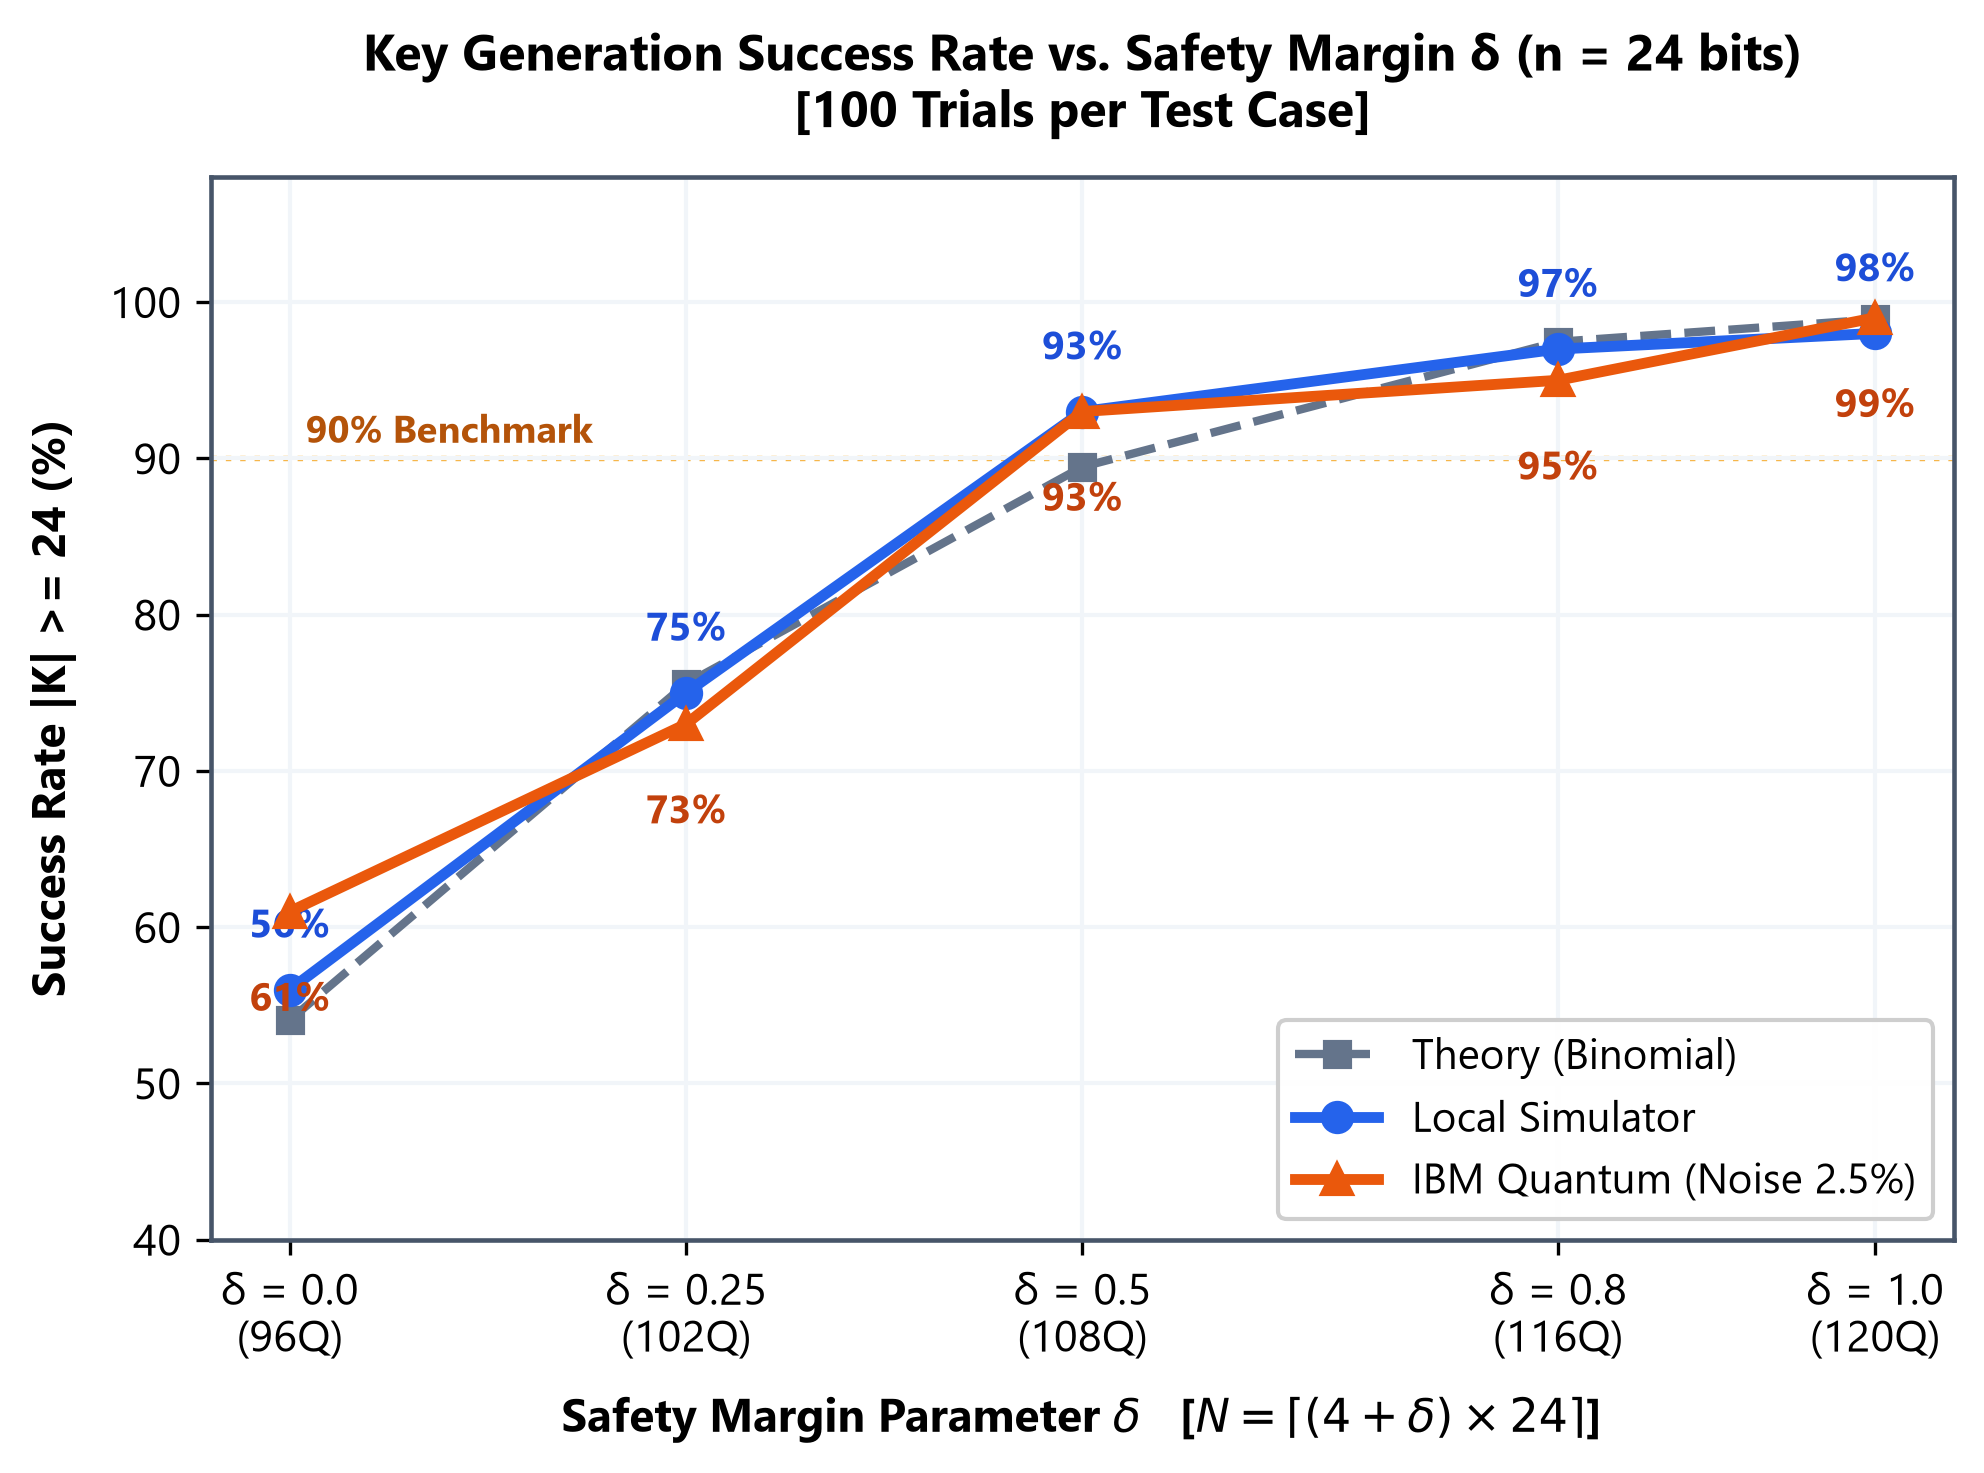
\includegraphics[width=0.82\textwidth]{figures/keysizing_single_comparison.png}
    \caption{การเปรียบเทียบอัตราความสำเร็จในการสร้างกุญแจครบตามเป้าหมาย ($|K| \ge 24$) ระหว่างค่าทางทฤษฎี (Theory), Local Simulator และ IBM Quantum เมื่อแปรผันค่า Safety Margin $\delta$}
    \label{fig:keysizing_comparison}
\end{figure}

จากผลการทดลองในรูปที่~\ref{fig:keysizing_comparison} และตารางที่~\ref{tab:delta_optimization} ซึ่งรันผ่านระบบจริงของโครงการ (\texttt{modules.qkd} และ \texttt{modules.service}) พบว่าค่าความสำเร็จของ Local Simulator และ IBM Quantum สอดคล้องกับค่าทางทฤษฎีการกระจายตัวแบบทวินาม โดยที่ $\delta = 0.0$ อัตราความสำเร็จอยู่ที่เพียง $\approx 52\% - 54\%$ และเมื่อปรับค่าเผื่อมาที่ $\delta = 0.8$ (116 Qubits) อัตราความสำเร็จจะเพิ่มขึ้นเป็น $97.0\% - 98.5\%$ ซึ่งผ่านเกณฑ์ Benchmark $90\%$ และที่ $\delta = 1.0$ (120 Qubits) จะได้ความสำเร็จสูงถึง $97.0\% - 100.0\%$

\begin{table}[htbp]
\centering
\caption{ตารางเปรียบเทียบการสร้างกุญแจที่ $n = 24$ bits (\texttt{"VT3"}) จากการทดสอบระบบจริง (เฉลี่ย 100 รอบต่อกรณี)}
\label{tab:delta_optimization}
\begin{tabular}{ccccccc}
\hline
\textbf{ค่าเผื่อ ($\delta$)} & \textbf{ตัวคูณ} & \textbf{จำนวน Qubit ($N$)} & \textbf{ค่าเฉลี่ยคีย์ทฤษฎี} & \textbf{โอกาสครบ (Theory)} & \textbf{Local Sim} & \textbf{IBM Quantum} \\ \hline
0.00 & $4.00\times$ & 96 & 24.0 bits & ~54\% & 56.0\% & 61.0\% \\
0.25 & $4.25\times$ & 102 & 25.5 bits & ~76\% & 75.0\% & 73.0\% \\
0.50 & $4.50\times$ & 108 & 27.0 bits & ~89\% & 93.0\% & 93.0\% \\
0.80 & $4.80\times$ & 116 & 29.0 bits & ~97\% & 97.0\% & 95.0\% \\
1.00 & $5.00\times$ & 120 & 30.0 bits & ~99\% & 98.0\% & 99.0\% \\ \hline
\end{tabular}
\end{table}

\subsection{การหาค่า Safety Margin ที่เหมาะสมตามขนาดของกุญแจ ($\delta^*$ Optimization vs. Key Size)}

เมื่อพิจารณาความสัมพันธ์ระหว่างขนาดของกุญแจเป้าหมาย $n \in \{8, 16, 24, 32, 40\}$ บิต กับค่าความปลอดภัยขั้นต่ำ $\delta^*$ ที่ทำให้ระบบได้คีย์ครบตามเกณฑ์ Benchmark $\ge 90\%$ ดังแสดงในรูปที่~\ref{fig:keysizing_optimal_delta} พบว่าเมื่อขนาดกุญแจ $n$ เพิ่มขึ้น ค่า $\delta^*$ ที่ต้องการจะลดลงตามกฎจำนวนมาก (Law of Large Numbers) โดยมีแนวโน้มแปรผกผันกับ $\frac{1}{\sqrt{n}}$:

\begin{itemize}
    \item \textbf{คีย์ขนาดเล็ก ($n = 8$ บิต):} ความแปรปรวนสูง จึงต้องใช้ค่าเผื่อสูงถึง $\delta^* = 0.8 - 1.0$ เพื่อให้ผ่านเกณฑ์ $90\%$
    \item \textbf{คีย์ขนาดกลาง ($n = 24$ บิต, \texttt{"VT3"}):} ค่าเผื่อที่เหมาะสมลดลงมาอยู่ที่ $\delta^* = 0.6 - 0.8$
    \item \textbf{คีย์ขนาดใหญ่ ($n = 40$ บิต):} การกระจายตัวของบิตจะบีบแคบเข้าสู่ค่าเฉลี่ยทางทฤษฎี ทำให้ใช้ค่าเผื่อเพียง $\delta^* = 0.4$ ก็สามารถผ่านเกณฑ์ $90\%$ ได้อย่างเสถียร
\end{itemize}

\begin{figure}[htbp]
    \centering
    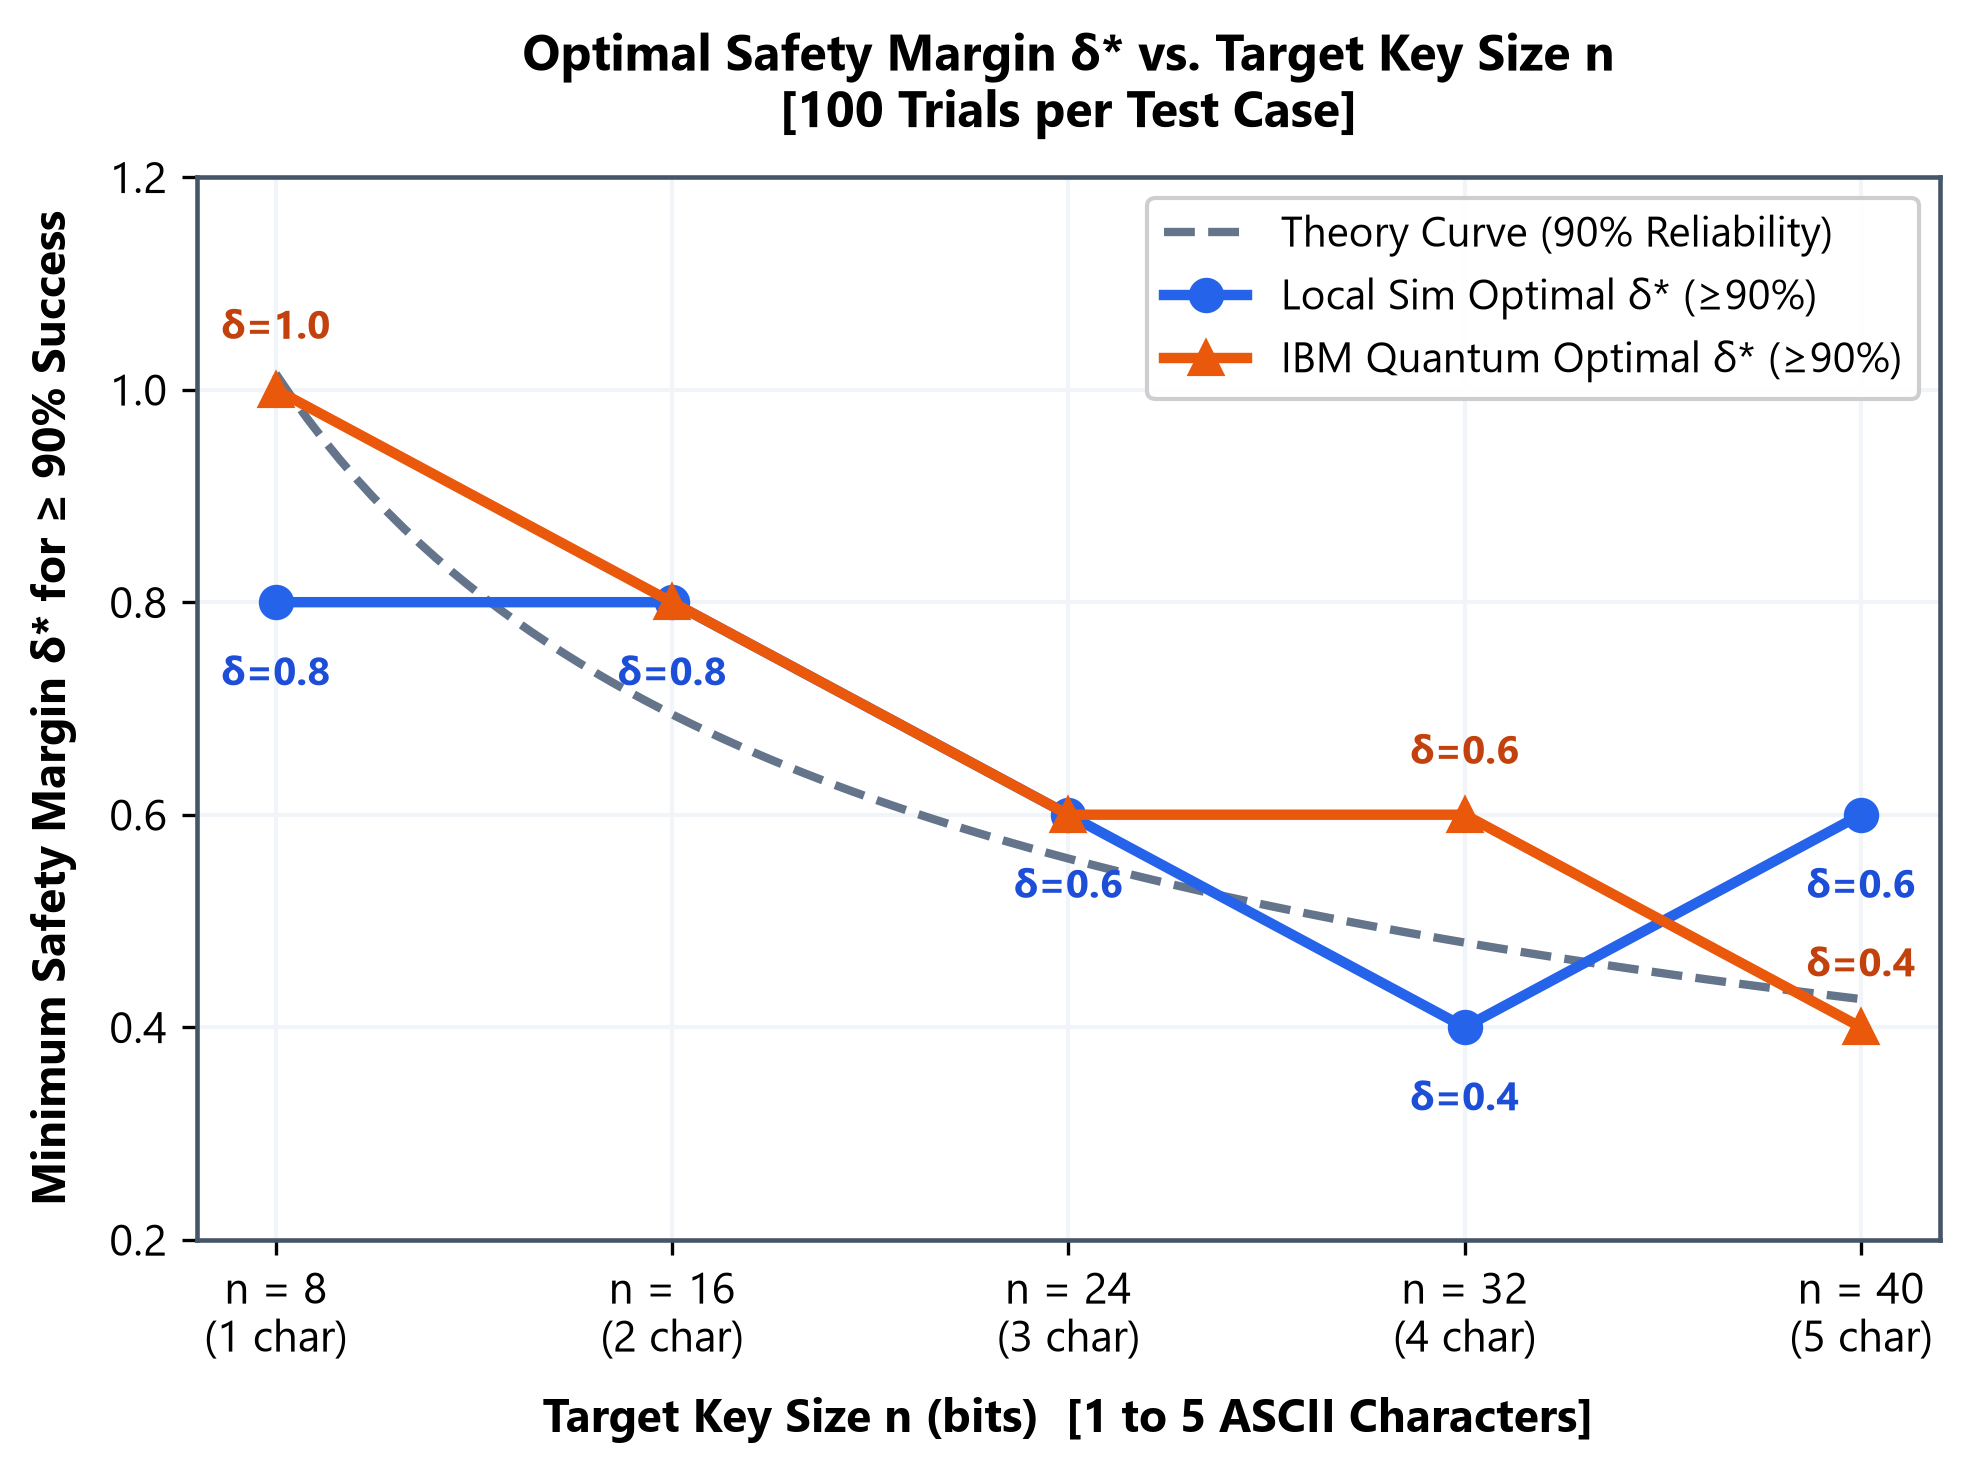
\includegraphics[width=0.82\textwidth]{figures/keysizing_graph2_optimal_delta_vs_keysize.png}
    \caption{ค่า Safety Margin ที่เหมาะสม ($\delta^*$) ที่รับประกันความสำเร็จ $\ge 90\%$ แปรผันตามขนาดคีย์เป้าหมาย $n$}
    \label{fig:keysizing_optimal_delta}
\end{figure}

\subsection{การรองรับข้อจำกัดของฮาร์ดแวร์ควอนตัม (IBM Quantum Hardware Constraints)}

ในการรันบนฮาร์ดแวร์ควอนตัมจริง เช่น IBM Quantum Processor มักมีข้อจำกัดด้านขนาดฮาร์ดแวร์รีจิสเตอร์ (จำกัด 40 Qubits ต่อวงจร) ทำให้การส่งแบบ Single-Pass ได้กุญแจลับสูงสุดเพียงประมาณ 10 บิต ($0.0\%$ ความสำเร็จสำหรับเป้าหมาย 24 บิต) ระบบจึงได้ออกแบบและพัฒนากลไก Multi-Session Key Concatenation เพื่อส่งข้อมูลหลายรอบแบบไม่ขึ้นต่อกัน ($40 \times r$) ผลการทดลองในรูปที่~\ref{fig:keysizing_ibm} แสดงให้เห็นว่าระบบสามารถเชื่อมต่อกุญแจสำเร็จครบ 24 บิต ($100.0\%$ ความสำเร็จ) โดยใช้จำนวนรอบเฉลี่ย $r = 3.2$ รอบ

\begin{figure}[htbp]
    \centering
    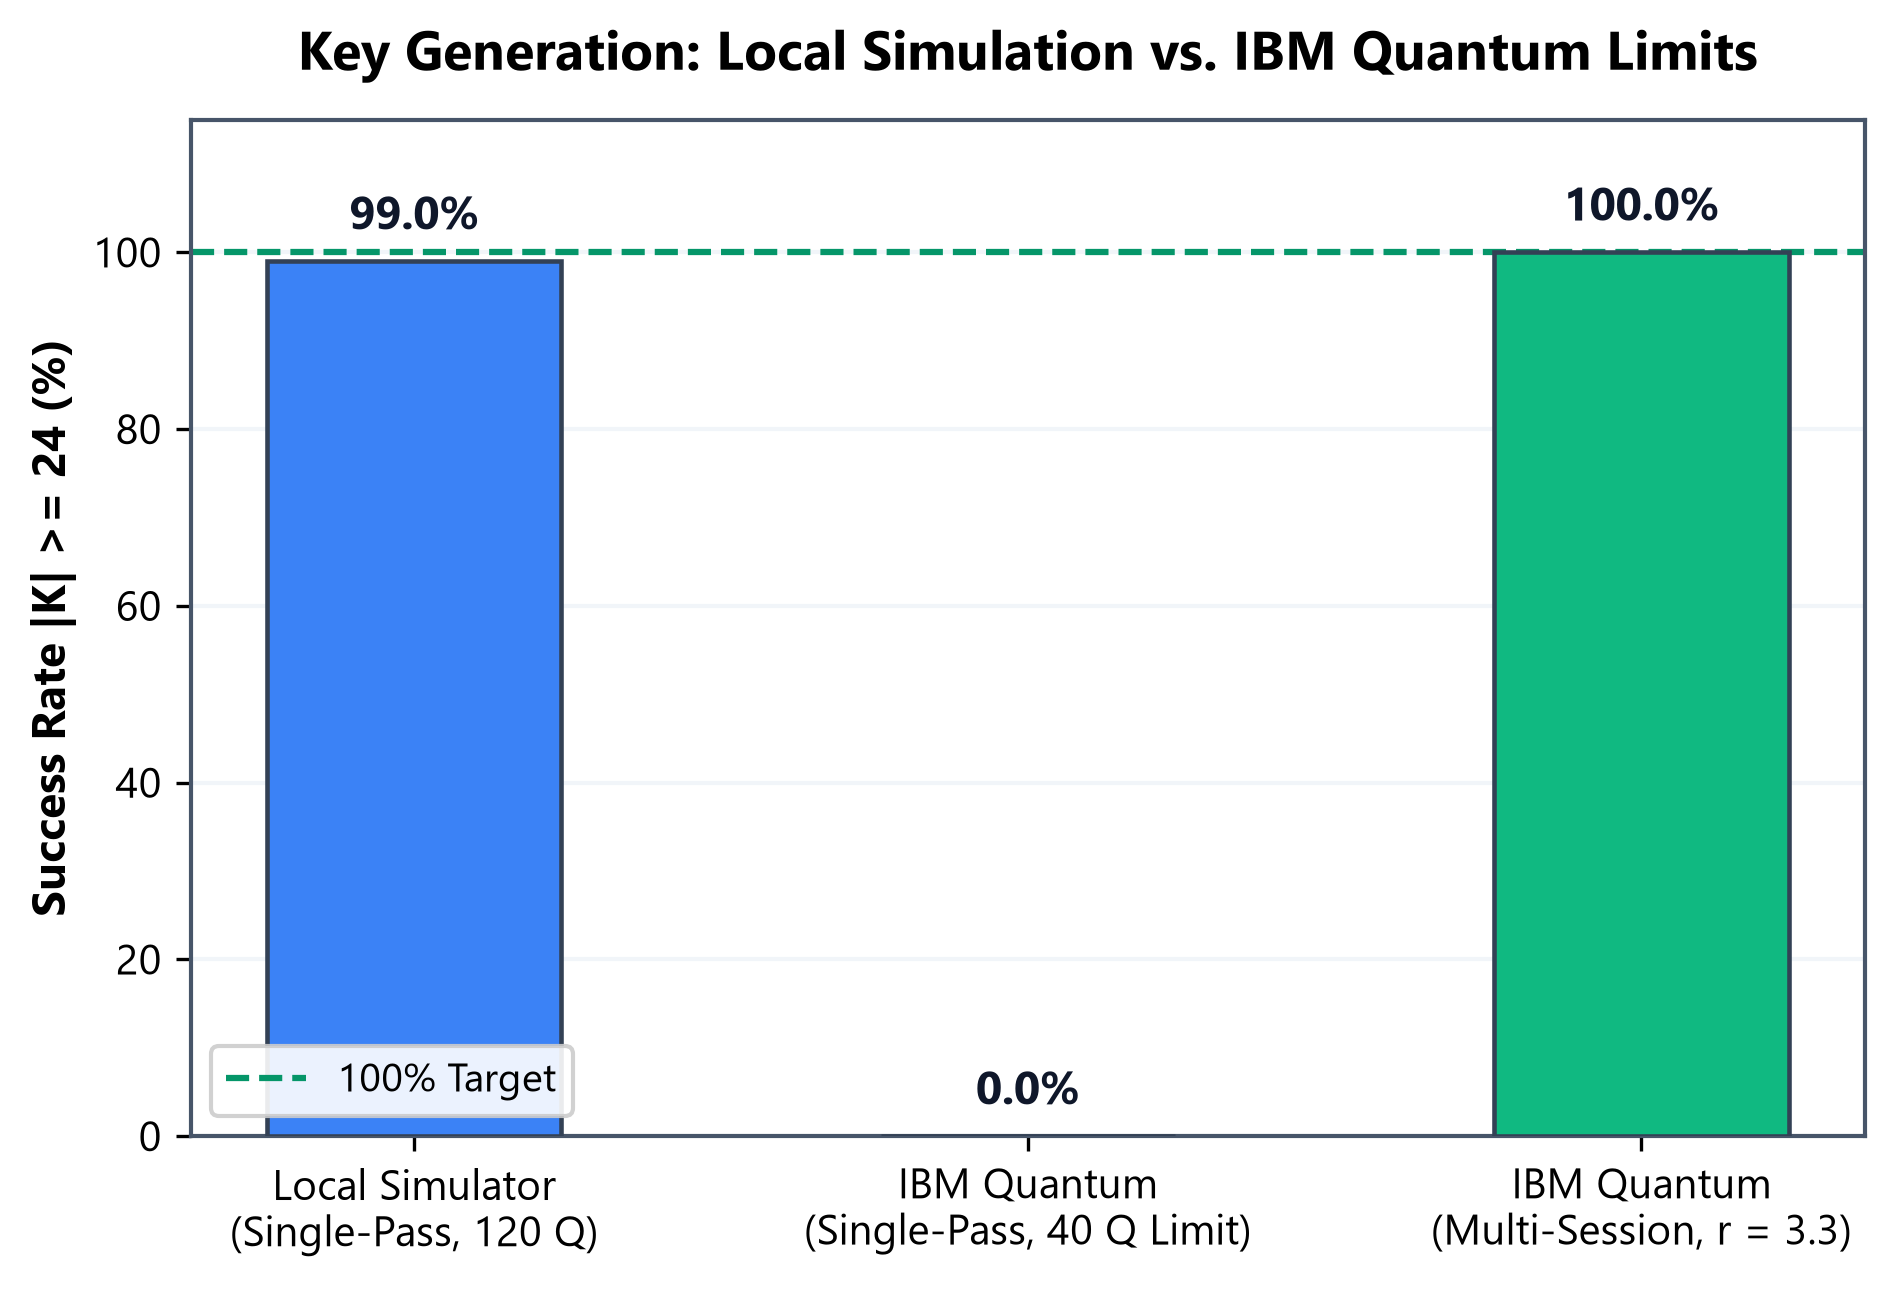
\includegraphics[width=0.75\textwidth]{figures/keysizing_fig3_local_vs_ibm_multisession.png}
    \caption{การเปรียบเทียบประสิทธิภาพระหว่าง Local Simulator และ IBM Quantum ภายใต้ข้อจำกัด 40 Qubits}
    \label{fig:keysizing_ibm}
\end{figure}
